\documentclass{article}

\usepackage{todonotes}

%\usepackage[disable]{todonotes}
\newcommand{\todot}[2][]{\todo[color=red!20!white,#1]{#2}}
\newcommand{\todof}[2][]{\todo[color=orange!20!white,#1]{#2}}


%%%%%%%%%%%%%%%%%%%%%%%%%%%%%%%%
% PACKAGES
%%%%%%%%%%%%%%%%%%%%%%%%%%%%%%%%
\usepackage{times}
\usepackage{fullpage}
\usepackage{latexsym}
\usepackage{amsmath}
\usepackage{amssymb}
\usepackage[boxed]{algorithm}
\usepackage{algpseudocode}
\usepackage{mathtools}
\usepackage{accents}
\usepackage{tikz}
\usepackage{pgfplots}
\usepackage{dsfont}
\usepackage[bf]{caption}
\usepackage{hyperref}
\hypersetup{
    bookmarks=true,         % show bookmarks bar?
    unicode=false,          % non-Latin characters in AcrobatÕs bookmarks
    pdftoolbar=true,        % show AcrobatÕs toolbar?
    pdfmenubar=true,        % show AcrobatÕs menu?
    pdffitwindow=false,     % window fit to page when opened
    pdfstartview={FitH},    % fits the width of the page to the window
    pdftitle={My title},    % title
    pdfauthor={Author},     % author
    pdfsubject={Subject},   % subject of the document
    pdfcreator={Creator},   % creator of the document
    pdfproducer={Producer}, % producer of the document
    pdfkeywords={keyword1} {key2} {key3}, % list of keywords
    pdfnewwindow=true,      % links in new window
    colorlinks=true,       % false: boxed links; true: colored links
    linkcolor=red,          % color of internal links (change box color with linkbordercolor)
    citecolor=blue,        % color of links to bibliography
    filecolor=magenta,      % color of file links
    urlcolor=cyan           % color of external links
}
\usepackage{comment}
\usepackage{amsthm}
\usepackage{natbib}
\usepackage[capitalize]{cleveref}
\usepackage{graphicx}
\usepackage{parskip}
\usepackage{tikz} 
\usetikzlibrary{arrows,positioning} 
\pgfarrowsdeclarecombine{ring}{ring}{}{}{o}{o}
\DeclareMathOperator{\ringarrow}{\raisebox{0.5ex}{\tikz[baseline]{\draw[ring->](0,0)--(2em,0);}}}
%%%%%%%%%%%%%%%%%%%%%%%%%%%%%%%%
% MACROS
%%%%%%%%%%%%%%%%%%%%%%%%%%%%%%%%
\newcommand{\defined}{\vcentcolon =}
\newcommand{\rdefined}{=\vcentcolon}
\newcommand{\E}{\mathbb E}
\newcommand{\Var}{\operatorname{Var}}
\newcommand{\calF}{\mathcal F}
\newcommand{\sr}[1]{\stackrel{#1}}
\newcommand{\set}[1]{\left\{#1\right\}}
\newcommand{\ind}[1]{\mathds{1}\!\!\set{#1}}
\newcommand{\argmax}{\operatornamewithlimits{arg\,max}}
\newcommand{\argmin}{\operatornamewithlimits{arg\,min}}
\newcommand{\floor}[1]{\left \lfloor {#1} \right\rfloor}
\newcommand{\ceil}[1]{\left \lceil {#1} \right\rceil}
\newcommand{\eqn}[1]{\begin{align}#1\end{align}}
\newcommand{\eq}[1]{\begin{align*}#1\end{align*}}
\newcommand{\Ber}{\operatorname{Bernoulli}}
\renewcommand{\P}[1]{\operatorname{P}\left\{#1\right\}}

\tikzset{
    %Define standard arrow tip
    >=stealth',
    %Define style for boxes
    observed/.style={
           circle,
           rounded corners,
           draw=black, thick,
           minimum width=2.5em,
           minimum height=2.5em,
           font=\footnotesize,
           text centered,
           fill=blue!20!white},
     latent/.style={
           circle,
           rounded corners,
           draw=black, thick, dashed,
           minimum width=.5em,
           minimum height=.5em,
           font=\footnotesize,
           text centered,
           fill=black!10!white
           },
     empty/.style={
           circle,
           rounded corners,
           minimum width=.5em,
           minimum height=.5em,
           font=\footnotesize,
           text centered,
           },
    % Define arrow style
    pil/.style={
           o->,
           thick,
           shorten <=2pt,
           shorten >=2pt,},
    sh/.style={ shade, shading=axis, left color=red, right color=green,
    shading angle=45 }  
}


%%%%%%%%%%%%%%%%%%%%%%%%%%%%%%%%
% THEOREMS
%%%%%%%%%%%%%%%%%%%%%%%%%%%%%%%%
\theoremstyle{plain}
\newtheorem{theorem}{Theorem}
\newtheorem{proposition}[theorem]{Proposition}
\newtheorem{lemma}[theorem]{Lemma}
\newtheorem{corollary}[theorem]{Corollary}
\theoremstyle{definition}
\newtheorem{definition}[theorem]{Definition}
\newtheorem{assumption}[theorem]{Assumption}
\newtheorem{remark}[theorem]{Remark}
\newtheorem{example}[theorem]{Example}



\begin{document}
\def\ci{\perp\!\!\!\perp}

\begin{comment}
\section{Random notes}
Information directed sampling have developed a general framework to construct algorithms that leverege generic structure between arms to minimize Bayesian regret, by explicitly trading off expected regret and information gain at each timestep. 

What can be expressed in the partial monitoring framework that cannot be defined by the feedback graph? 

 

We consider a variant of the stochastic multi-armed bandit problem when we have prior knowledge of the causal structure, but not the functional form, of the relationship between variables. 


sequential decision process,exploration-exploitation trade off 



Points to present. Why we use regret against single best arm - it makes sense in the stochastic setting. 
The difference between observational and interventional distributions. 

terminology for intervention vs observation. Recast bandit algorithm in terms of this. Show limitations to existing approaches by pointing to places were existing algorithms eg UCB/explore-exploit/exp3 require unbiased estimates. Are unbiased estimates actually impossible in our setting?

This paper is about sequentially choosing actions. 
Modelling sequntial decition processes. 

In the classic multi-armed bandit setting, an ag

General bandit part ... define multi-armed bandit, and importance. Decision making is fundamental. Goal is to select an action to maximize a reward (or minimize a loss). In many settings, such as drug trials, online ad placement, etc we can choose actions sequentially. This introduces an exploration-exploitation trade-off. 

The problem of sequentially choosing actions to minimize some loss wide range of applications in XXXX, YYYY. The multi-armed bandit setting, in which .... . 

Now the required causal stuff should go here. 

Causal structure can be represented as a directed acyclic graph with nodes representing the variables and an edge from $A \rightarrow B$ meaning $A$ causes $B$. Deterministic interventions, consisting of setting variables to some value, are modelled by setting the nodes to the desired values and removing any links coming into them, as their value is now no longer set by other variables in the graph according to the original mechanism. 

If the causal graph is known, such that there are no hidden variables causing 2 or more of the variables and the probabilities are all > 0 then the distribution of any variable after any intervention can be inferred (asymptotically) from data collected in absence of any interventions.
\end{comment}

\section*{Introduction}

Problems requiring choosing an action under uncertainty are rife in all areas of human endeavour. For many problems, actions may be chosen sequentially, allowing the agent to learn from the outcome of early choices to improve later ones. A widely used framework for sequential decision making is the multi-armed bandit. In the classic multi-armed bandit setting there is a finite set of available actions, each associated with a distribution over rewards which is unknown but stationary and independent of the reward distribution of other actions. At each timestep the agent selects an action and receives a reward sampled iid from the corresponding reward distribution.  

An an alternate approach to selecting actions is causal inference. Frameworks for causal inference provide a mechanism to specify assumptions that allow observational distributions over variables to be mapped to interventional ones. This allows an agent to predict the outcome of an action based on non-experimental data. This approach is common in social science, demography, and economics where explicit experimentation may be difficult. For example, predicting the effect of changes to childcare subsidies on workforce participation or school choice on student grades. 

We take a first step towards unifying these approaches by considering a variant of the stochastic multi-armed bandit problem where we have prior knowledge of the causal structure governing the available actions. This structure creates dependencies between the rewards of different arms such that selecting one action can provide information on the reward for other actions. 

There has been substantial recent work into extending bandit algorithms to incorporate additional assumptions and deal with more complex feedback structures. Algorithms with strong guarantees have been developed for linear bandits [], generalized linear bandits, gaussian process bandits [], etc. There is also an active line of research into bandits with feedback defined by a graph. Actions are modelled as nodes in the graph and the agent observes rewards for each action connected to the selected action []. The novelty of our work is that we assume prior knowledge of the causal structure but not the functional form of the relationship between variables. 


\section*{Problem Formulation}
Assume we have a known causal model with binary variables $\boldsymbol{X} = \{X_{1}..X_{N}\}$ that independently cause a target variable of interest $Y$, figure \ref{fig:causalStructure}. We can run sequential experiments on the system, where at each timestep $t$ we can select a variable on which to intervene and subsequently observe the complete result, $(\boldsymbol{X}_{t},Y_{t})$. As an example, consider a farmer wishing to optimize the yield of her crop. She can invest in a green house to control temperature, a watering system to control soil moisture, fertilizers to set soil nutrients, etc. We assume only a single intervention is feasible due to cost and that each of these variables are independent of one-another (this may not always be the case - temperature could be related to rainfall for example). After having selected which variable to control, she plants her crops and observes the values of the remaining input variables and the yield. This repeats across many growing seasons, and the goal is to maximize the total cumulative yield.

\begin{figure}[h]
\centering
\caption{Assumed Causal Structure}
\label{fig:causalStructure}
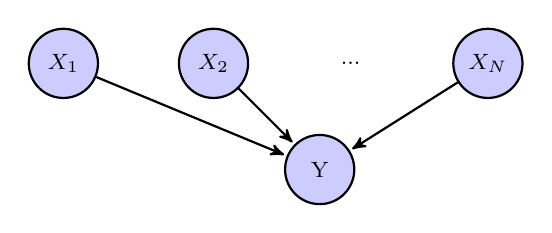
\begin{tikzpicture}[->,>=stealth',shorten >=1pt,auto,node distance=1cm,
  thick,main node/.style={observed}, hidden/.style={empty}]

 %nodes
\node[main node](1){$X_{1}$};
\node[main node, right=of 1](2){$X_{2}$};
\node[hidden, right=of 2](3){$...$};
\node[main node, right=of 3](4){$X_{N}$};
\node[main node, below right=of 2](5){Y};
 \path[every node/.style={font=\sffamily\small}]
    (1) edge (5)
    	(2) edge (5)
    (4) edge (5);
	
\end{tikzpicture}
\end{figure}


Let $q \in [0,1]^N$ be a fixed vector where $q_i = P(X_i = 1)$. In each time-step $t$ upto a known end point $T$:
 
\begin{enumerate}
\item The learner chooses an $I_t \in \set{1,\ldots, N}$ and $J_t \in \set{0,1}$.
\item Then $X_t \in \set{0,1}^N$ is sampled from a product of Bernoulli distributions, $X_{t,i} \sim \Ber(q_i)$ 
\item The learner observes $\tilde X_t \in \set{0,1}^K$, which is defined by 
\eq{
\tilde X_{t,i} = \begin{cases}
X_{t,i} &\text{if } i \neq I_t \\
J_t & \text{otherwise}\,.
\end{cases}
}
\item The learner receives reward $Y_t \sim \Ber(r(\tilde X))$ where $r:\set{0,1}^K \to [0,1]$ is unknown and arbitrary.
\end{enumerate}

The expected reward of taking action $i,j$ is $\mu_{i,j} = \E[r(X)|do(X_i = j)]$. The optimal reward and action are denoted $\mu^*$ and $(i^*,j^*)$ respectively,
where $(i^*,j^*) = \argmax_{i,j} \mu_{i,j}$ and $\mu^* = \mu(i^*,j^*)$. The $n$-step cumulative expected regret is
\eq{
R_n = \E \sum_{t=1}^n \left(\mu^* - \mu_{I_t,J_t}\right).
}

The problem can be treated as a classical multi-armed bandit with $K = 2N$ arms. However, this does not utilize the information provided by the causal assumption. 

Now need to expand upon how the assumption gives us extra information. 

The difficulties faced due to bias.

To deal with this issue we use a simple explore-exploit algorithm. Our algorithm will explore for $h$ time-steps, sampling actions in a way that depends on our prior knowledge of $q$ but is independent of the observed rewards. We then select the arm with the highest expected reward for the remaining $T-h$ time steps. 

\section{Bounding the Simple Regret}

\begin{itemize}
\item $N$ is number of variables.
\item $q_i$ is probability that $X_{i,t} = 1$ for any $t$
\item $s_i = \min\set{q_i, 1 - q_i}$
\item $h = T/2$
\item $\mu : \set{1,\ldots,N} \times \set{0,1} \to [0,1]$.
\item $I_t \in \set{1,\ldots,N} \times \set{0,1}$ is the intervention
\end{itemize}

Let $r_T$ be the simple regret after $T$ time steps, which is
\eq{
r_q(T) = \E\left[\mu^* - \mu_{I_T}\right]\,,
}
where $\mu^*$ is the mean payoff of the optimal intervention and $I_T$ is the intervention chosen in the $T$th round.
We propose a two part algorithm that is provably order optimal when its performance is measured in terms of the simple regret.


\begin{algorithm}[H]
\caption{Simple Regret Algorithm}\label{alg:simple}
\begin{algorithmic}[1]
\State {\bf Input:} $T, N$
\State $h = T/2$
\For{$t \in 1,\ldots,h$}
\State Do nothing and observe $X_{i,t}$ for $i \in \set{1,\ldots,N}$ and $r_t$
\EndFor
\State Compute for all $i \in \set{1,\ldots,N}$ and $j \in \set{0,1}$:
\eq{
\hat \mu_{i,j} = \frac{\sum_{t=1}^h \ind{X_i = j} r_t}{\sum_{t=1}^h \ind{X_i = j}}\,.
}
\State Compute $\hat q_i = \frac{1}{h} \sum_{t=1}^h X_{i,t}$
\State Compute $\hat s_i = \min\set{\hat q_i, 1 - \hat q_i}$
\State Compute $\hat{s'} = sorted(\hat{s}) : \hat{s'}_1 \leq \hat{s'_2} \leq ... \leq \hat{s'}_N$
\State Compute $\hat m = \min\set{2 \leq i \leq N : \hat s'_{i} \geq 1/i}$
\State $i'(i) = $ the index of $\hat s_i$ in $\hat s'$
\State Compute $A$ as the subset of infrequently observed arms $\{(i,j):i'(i) \leq \hat m, j = \ind{\hat q_{i} \leq \frac{1}{2}} \}$ with $|A| = \hat m$

\For{$(i,j) \in A$}
\For{$t \in 1,\ldots,h/\hat m$}
\State Choose $I = i$ and $J = j$
\State Observe reward $r_t$
\EndFor
\State Recompute $\hat \mu_{i,j} = \frac{\hat m}{h} \sum_{t=1}^{\hat m/h} r_t$ 
\EndFor
\end{algorithmic}
\end{algorithm}

\begin{theorem}\label{thm:simple-regret}
Define $m = \min\set{2 \leq i \leq N : q_i \geq 1/i}$.
Then the algorithm given in \cref{alg:simple} satisfies
\eq{
r_q(T) \in O\left(\sqrt{\frac{m}{T} \log \left(\frac{NT}{m}\right)}\right)\,.
}
\end{theorem}

\begin{lemma}\label{lem:conc1}
$\displaystyle \P{\left|\hat q_i - q_i\right| \geq \sqrt{\frac{3q_i}{h} \log \frac{2}{\delta}}} \leq \delta$.
\end{lemma}

\begin{proof}
Let $Z_t = \ind{X_{i,t} = 1} \in \set{0,1}$.
Then
\eq{
\hat q_i = \frac{1}{h} \sum_{t=1}^{h} Z_t\,.
}
Now $Z_1,\ldots,Z_h$ is an i.i.d.\ sequence of Bernoulli random variables with with mean $q_i$. The result follows from the Chernoff bound.
\end{proof}

\begin{lemma}\label{lem:conc2}
Let $\delta >0$ and $\hat s_i = \min\set{\hat q_i, 1 - \hat q_i}$ and
define $\hat m = \min\set{2 \leq i \leq N : \hat s_{(i)} \geq 1/i}$.
If
\eq{
h \geq 12m \log\frac{2N}{\delta}\,,
}
then
\eq{
\P{\hat m \leq 2m} \geq 1 - \delta\,.
}
\end{lemma}

\begin{proof}
It is easy to see that the worst case occurs when 
\eq{
q_i = \begin{cases}
0 & \text{if } i < m \\
\frac{1}{m} & \text{otherwise}\,.
\end{cases}
}
Now by \cref{lem:conc1} we have with probability at least $1 - \delta$ that 
\eq{
(\forall i) \qquad \left| \hat q_i - q_i\right| 
&\leq \sqrt{\frac{3q_i}{h} \log \frac{2N}{\delta}} \\
&= \sqrt{\frac{3}{mh} \log\frac{2N}{\delta}}\,. 
}
By assumption 
\eq{
h \geq 12m \log \frac{2N}{\delta}\,.
}
Therefore with probability at least $1 - \delta$ we have
\eq{
(\forall i) \qquad \left|\hat q_i - q_i\right| \leq \frac{1}{2m}\,.
}
Note that for $i$ with $q_i = 0$ it is easy to see that $\hat q_i = 0$ (the variance is zero). The above guarantee that
for $i$ with $q_i = 1/m$ we have $\hat q_i \in [1/(2m), 3/(2m)]$ for all $i$ with probability at least $1 - \delta$,
which implies that $\hat s_i \geq 1/(2m)$ for all $i$ where $q_i = 1/m$.
Therefore $\hat m \leq 2m$ with probability at least $1 - \delta$. 
\end{proof}


\begin{proof}[Proof of \cref{thm:simple-regret}]
Given the assumption that
\eq{
h \geq 12m \log \frac{N}{\delta}
}

\eq {
\text{ for } (i,j)\in A \qquad \hat \mu_{i,j} = \frac{\hat m}{h} \sum_{t=1}^{\hat m/h} r_t
}
Prove bound for this case

\eq {
\text{ for } (i,j)\notin A \qquad \hat \mu_{i,j} = \frac{\sum_{t=1}^h \ind{X_i = j} r_t}{\sum_{t=1}^h \ind{X_i = j}}
}

Prove bound for this case


we have shown with probability at least $1 - \delta$ that
\eq{
(\forall i, j) \qquad \left|\hat \mu_{i,j} - \mu_{i,j}\right| \leq \sqrt{\frac{m}{h} \log\frac{N}{\delta}}\,.
}
Suppose $h < 12m \log \frac{N}{\delta}$. Then
\eq{
\left|\hat \mu_{i,j} - \mu_{i,j}\right| \leq 1 \leq \sqrt{\frac{12m}{h} \log \frac{N}{\delta}}\,.
}
Therefore
\eq{
\left|\hat \mu_{i,j} - \mu_{i,j}\right| \leq \sqrt{\frac{12m}{h} \log \frac{N}{\delta}}\,.
}
Therefore 
\eq{
r_q(T) 
&\leq \delta + \sqrt{\frac{12m}{h} \log \frac{N}{\delta}} \\
&= \delta + \sqrt{\frac{24m}{T} \log \frac{N}{\delta}} \\
&\leq \frac{m}{T} + \sqrt{\frac{24m}{T} \log \left(\frac{NT}{m}\right)}
}
as required.
\end{proof}

\section*{Results}

Summarize results here and note differences to classic bandit results

\subsection*{Known and Balanced q}

We begin with the simplest case were we assume that $q_i=\frac{1}{2} \forall i$. During the exploration phase we sample actions uniformly at random. In this case, this is equivalent to purely observing, that is taking no action and allowing all input variables to take their value randomly as  $X_{t,i} \sim \Ber(\frac{1}{2})$. 



We will have $n_i \sim Binomial(h,\frac{1}{2})$ observations for each arm $i$ at the end of the exploration stage. Note that this is independent of the number of arms $K$.



Assume we have $K$ bernoulli arms with means ordered from highest to lowest $\mu_1 ... \mu_K$. Let $\Delta = [\Delta_1...\Delta_K]$ be the differences from the optimal reward $\mu_1$. 



 

\subsubsection*{Regret during explore phase}
Since the probability we play each arm is constant and uniform during the exploration phase, the expected regret is simply proportional to the average sub-optimality $\Delta$.
\eqn{
R_1 = h\sum_i P(i)\Delta_i = \frac{h}{K}\sum_i \Delta_i = h E[\Delta]
}

\subsubsection*{Regret during exploit phase}
The regret during this phase is proportional to the expected sub-optimality of the arm with the highest empirical mean at the end of the explore phase.

\eqn{
\hat{i^*} = argmax_i [\hat{\mu}_i]
}
\eqn{
R_2 = (T-h)E[\Delta_{\hat{i^*}}] = (T-h)\sum_i P(\hat{\mu}_i \geq \hat{\mu}_j \forall j)\Delta_i 
}

The difficulty with this approach is that it is hard to get bounds that are tight for all $\Delta$. Instead, we will bound the probability that we select an arm with a sub-optimality gap greater than some $D$.
\eqn{
R_2 \leq (T-h)\left(P(\Delta_{\hat{i^*}} \leq D) D+P(\Delta_{\hat{i^*}} > D)  \Delta_{max} \right)
}
The goal now is to get a bound for $P(\Delta_{\hat{i^*}} > D)$ in terms of Hoeffdings type bounds for each arm. 

Suppose $i = \hat{i^*} \implies \hat{\mu}_i > \hat{\mu}_1$. If we haven't over-estimated $\mu_i$ too much, $\hat{\mu}_i - \mu_{i} < \frac{D}{2}$, and haven't under-estimated $\mu_1$ too much, $\mu_1 - \hat{\mu_1} < \frac{D}{2}$, then $\Delta_{\hat{i^*}} = \mu_1 - \mu_i < D$

\eqn{
\label{eqn:probDeltaToLarge}
P(\Delta_{\hat{i^*}} > D) \leq  P(\mu_1 - \hat{\mu_1} > \frac{D}{2})+ \sum_{i=2}^K P(\hat{\mu}_i - \mu_{i} > \frac{D}{2})
}

If we used the empirical mean as an estimator for $\mu_i$, the bound will depend on the number of times we actually observed each arm, which will be a random variable drawn from a multinomial distribution. Instead we will use an importance weighted estimator.

\eqn{
\label{eqn:importance_weighted_estimator}
\hat{\mu}_i = \frac{1}{h}\sum_{t=1}^h \frac{Y_t\ind{\text{arm $i$ active}}}{q_i}
}

where $q_i = P(\text{arm $i$ active})$

Hoeffdings gives $ P(\hat{\mu}_i - \mu_{i} > \epsilon) \leq e^{-2h\epsilon^2q_i^2}$. In this case we have assumed $q_i = \frac{1}{2} \forall i$. Putting this into equation \ref{eqn:probDeltaToLarge}:

\eqn{
\label{eqn:balancedHoeffdings}
P(\Delta_{\hat{i^*}} > D) \leq Ke^{-hD^2/8}
}


\eqn{
R_2 \leq (T-h)[(1-K e^{-hD^2/8})D + K e^{-hD^2/8}] < (T-h)[D + K e^{-hD^2/8}]
}

Let $D = \sqrt{\frac{8}{h}\log(hK)}$ 

\eqn{
R_2 \leq (T-h)\left(\sqrt{\frac{8}{h}\log(hK)} + \frac{1}{h}\right)
}


\subsection*{Total Regret}

Putting together the regret from the exploration and exploitation phases,

\eqn{
R_T & \leq \frac{h}{K}\sum_i \Delta_i + (T-h)\left(\sqrt{\frac{8}{h}\log(hK)} + \frac{1}{h}\right)\\
& \leq h + T\left(\sqrt{\frac{8}{h}\log(TK)} + \frac{1}{h}\right)
}

Now if we let $h = T^{2/3}(\log(KT))^{1/3}$,


\eqn {
R_T \leq 4T^{\frac{2}{3}}(log(KT))^{\frac{1}{3}} + T^{\frac{1}{3}}(log(KT))^{-\frac{1}{3}}
}

If $T \geq 2$ and $K \geq 2$, the first term dominates and,

\eqn {
R_T  \leq 5T^{\frac{2}{3}}(log(KT))^{\frac{1}{3}}
}

The distribution independent lower bound for optimised UCB is $O(\sqrt{TK})$ (see Bubeck sect 2.4.3) so we would expect our algorithm to do better if $K >> T^{\frac{1}{3}}$



\subsection*{Empirical results}
\begin{figure}[H]
\centering
\caption{Comparison of the UCB and causal-explore-exploit for K=20 and T=10000. Note, $K \sim T^{1/3}$ Plot shows average and standard deviation over 10000 trials.}
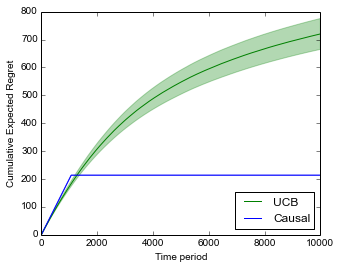
\includegraphics[width=.5\textwidth]{explore_exploit}
\end{figure}

\section{Generalizing to unbalanced $\boldsymbol{q}$}

When some arms have low natural probability we cannot rely on exploring them adequately by pure observation. We need to explicitly play them during the exploration phase. 

We now have an additional trade off to make, which is how much should be observe (learning something about at least half the arms each timestep) versus playing the low probability arms. 

Without loss of generality, we can assume $q_i \in [0,\frac{1}{2}]$ and $q_1 \leq q_2 ... \leq q_N$. Let $m \in [2,N] = \{m:q_m > \frac{1}{m}\}$ Ie if the problem is completely balanced $q_1...q_N = \frac{1}{2}$ then $m = 2$. If the problem is completely unbalanced, $q_1...q_N = 0$ then $m=N$

Suppose we observe for the first $h/2$ timesteps. This is at worst half the optimal. 

We then have estimates 

\eqn {
\hat{\mu}_{ij} = \frac{\sum_{t=1}^{h/2}\ind{Y=1,X_i=1}}{\frac{h}{2}q_{ij}}
}

We take this as our estimate for those arms for which $q_{ij} > \frac{1}{m}$

For these arms the Hoeffdings gives 

\eqn{
P(\hat{\mu}_i - \mu_{i} > \frac{D}{2}) \leq e^{-hD^2/2m^2}
}

We play each of the remaining $m$ arms $\frac{h}{2m}$ times so for them we get

\eqn{
P(\hat{\mu}_i - \mu_{i} > \frac{D}{2}) \leq e^{-hD^2/4m}
}

So for all the arms 

\eqn{
P(\hat{\mu}_i - \mu_{i} > \frac{D}{2}) \leq e^{-hD^2/4m^2}
}

and 



\eqn{
\label{eqn:unbalancedHoeffdings}
P(\Delta_{\hat{i^*}} > D) \leq Ke^{-hD^2/4m^2}
}

If we let $D = \sqrt{\frac{4m^2\log(hK)}{h}}$

\eqn{
R_T  \leq h + T\left(\sqrt{\frac{4m^2\log(hK)}{h}} + \frac{1}{h}\right)
}

Let $h = T^{2/3}m^{2/3}\log(hk)$


\eqn {
R_T  \leq 4T^{\frac{2}{3}}m^{2/3}(log(KT))^{\frac{1}{3}}
}

Note, I think the $m^{2/3}$ should be improvable to something close to $m^{1/3}$ is I use Berstein's instead of Hoeffdings to bound the estimator for the arms where $q > 1/m$ but I haven't got the equations to quite work out for that yet. 

It should also be possible to generalize to handle the case were the $q$'s are unknown, since we should be able to get a reasonable estimate for them while we are observing. They key will be how the resulting uncertainty in $m$ effects the bounds. 

To get results that degrade to similar order bounds as UCB when the arms are very unbalanced, I will need to drop the explore/exploit strategy. 


\subsection{Generalizing to unknown q}
We now consider the case where $\boldsymbol{q}$ is not known in advance. Assume as before that we observe for $h/2$ timesteps. From the observations gained in this phase we estimate $\boldsymbol{q}$.

\eqn{
\hat{q}_i = \frac{2}{h}\sum_{t=1}^{h/2}\ind{X_i=1}
}

Let $\bar{q}_i = min(\hat{q},1-\hat{q})$ and construct $\bar{\boldsymbol{q}}$ such that $\bar{q}_1 \leq \bar{q}_2 \leq ...\leq \bar{q}_N$. We then estimate $m$ with $\hat{m} = min_i : \bar{q}_i \geq \frac{1}{i}$  

We estimate the reward for the apparently common arms, $i \geq \hat{m}$, as:

\eqn{
\hat{\mu}_i = \frac{\sum_{t=1}^{h/2}\ind{Y = 1,X_i = 1}}{\frac{h}{2}\hat{q}_i} = \frac{\sum_{t=1}^{h/2}\ind{Y = 1,X_i = 1}}{\sum_{t=1}^{h/2}\ind{X_i=1}}
}

We play the remaining arms $\frac{h}{2\hat{m}}$ times and estimate their reward as:

\eqn{
\hat{\mu}_i = \frac{2\hat{m}}{h}\sum_{t=1}^{h/2\hat{m}}\ind{Y = 1|X_i=1}
}

We now consider how errors in the estimation of $m$ effect our estimates of the arm rewards. For the arms with $i \geq \hat{m}$ we know $\hat{q}_i \geq \frac{1}{\hat{m}}$ and thus our estimate is based on at least $\frac{h}{2\hat{m}}$ observations. Similarly we explicitly play the infrequently observed arms, $i < m$,  $\frac{h}{2\hat{m}}$ times. Thus our estimates will only be worse than the known $\boldsymbol{q}$ case if $\hat{m} > m$. 

For a fixed $m$ the $\boldsymbol{q}$ most likely to lead us to overestimate $m$ is: \todot{Justify this claim.}


\eqn{
q_i = \begin{cases}
0 & \text{ if } i < m\\
\frac{1}{m} & \text{ if } i \geq m
\end{cases}
}

We now bound $P(\hat{m} - m > \varphi)$ for this worst case.



For $i < m$,we have $\bar{q}_i = q_i = 0$. For $i \geq m$ \todot{Is this really true, justify}
\eq{
P(q_i - \bar{q}_i \geq C) & =  P(q_i - \hat{q}_i \geq C|\hat{q}_i\leq \frac{1}{2})P(\hat{q}_i \leq \frac{1}{2})+P(q_i - (1-\hat{q}_i) \geq C | \hat{q}_i > \frac{1}{2})P(\hat{q}_i>\frac{1}{2})\\
& \leq  2P(q_i - \hat{q}_i \geq C|\hat{q}_i\leq \frac{1}{2})
}

 
Via Bernstein's Inequality:
\eqn{
&2P(q_i - \hat{q}_i \geq C | \hat{q}_i \leq \frac{1}{2}) \leq 2\exp(-\frac{hC^2}{4q_i}) := \gamma \\
\implies &P(q_i - \hat{q}_i \geq 2\sqrt{\frac{\log(2/\gamma)}{mh}})\leq \gamma
}

Define $\hat{m}_i = \frac{1}{\hat{q}_i}$.

\eqn{
\hat{q}_i \geq q_i - C & \implies \hat{m}_i \leq \frac{1}{q_i-C} = \frac{1}{\frac{1}{m} - C} \text{, where } C < \frac{1}{m} \\
& \implies q_i - \hat{q}_i \leq C \implies \hat{m}_i - m \leq \frac{m^2C}{1-mC}\\
& \implies P(\hat{m}_i - m \geq \frac{m^2C}{1-mC}) \leq \gamma
}

Let $\varphi = \frac{m^2C}{1-mC} \implies C = \frac{\varphi}{m(\varphi+m)} \implies \gamma = 2\exp(-\frac{h \varphi^2}{4m(\varphi+m)^2}) \implies \varphi = \frac{2m\sqrt{m\log(2/\gamma)}}{\sqrt{h}-2\sqrt{m \log(2/\gamma)}} $

Note this implies that if $h \geq 16m\log(2/\gamma)$ then $\varphi \leq m$

\eqn {
P(\hat{m}_i - m \geq \varphi) \leq 2\exp(-\frac{h \varphi^2}{4m(\varphi+m)^2})
}


If $\hat{m}_i - m \geq \varphi$ for at most $\varphi$ of the variables $i \geq m$, then $\hat{m} - m \leq \varphi$

Let $W_i = \ind{\hat{m_i}-m \geq \varphi}$, $E[W_i] \leq \gamma$,$V[W_i] \leq \gamma$ 
\eqn{
P(\sum_{i=m}^N W_i \geq (N-m)\gamma + \varepsilon) \leq \exp(-\frac{\varepsilon^2}{2(N-m)\gamma+2\varepsilon/3})
}
Letting $(N-m)\gamma + \varepsilon = \varphi \implies \varepsilon = \varphi - (N-m)\gamma$
\eqn{
P(\hat{m}-m \geq \varphi) =  P(\sum_{i=m}^N W_i \geq \varphi) &\leq \exp({-\frac{(\varphi-(N-m)\gamma)^2}{2(N-m)\gamma + 2(\varphi-(N-m)\gamma)/3}})\\
& \leq \exp({-\frac{(\varphi-N\gamma)^2}{2N\gamma + 2\varphi/3}}) \text{, where } N\gamma < \varphi
} 



If $P(\hat{m}-m \geq \varphi) \leq \zeta$. 


\eqn{
P(\hat{\mu}_i-\mu_i \geq \epsilon) \leq & P(\hat{\mu}_i-\mu_i \geq \epsilon |\hat{m}-m \leq \varphi )P(\hat{m}-m \leq \varphi) \\
& + P(\hat{\mu}_i-\mu_i \geq \epsilon |\hat{m}-m \geq \varphi)P(\hat{m}-m \geq \varphi)\\  \leq & e^{-\frac{h\epsilon^2}{m+\varphi}} + \zeta e^{-\frac{h \epsilon^2}{N}}
}

Putting it together 

\eqn {
P(\hat{\mu}_i-\mu_i \geq \epsilon)& \leq \exp({-\frac{h\epsilon^2}{m+\varphi}}) + \exp({-\frac{(\varphi-N\gamma)^2}{2N\gamma + 2\varphi/3}}) \exp({-\frac{h \epsilon^2}{N}})\\
& \leq \exp({-\frac{h\epsilon^2}{m+\varphi}}) + \exp({-\frac{(\varphi-N\gamma)^2}{2N\gamma + 2\varphi/3}}) \\
& \leq \exp({-\frac{h\epsilon^2}{m+\varphi}}) + \exp({-\frac{(\varphi-N\exp(-\frac{h\varphi^2}{4m(\varphi+m)^2}))^2}{2N\exp(-\frac{h\varphi^2}{4m(\varphi+m)^2}) + 2\varphi/3}})
}

Assume $h > 16m\log(2N)$ and . Let $\varphi = \epsilon\sqrt{h}$. Assume $\epsilon \geq \frac{m}{\sqrt{h}}$ so as to ensure $\varphi > m$
\eqn{
P(\hat{\mu}_i-\mu_i \geq \epsilon)& \leq \exp({-\frac{h\epsilon^2}{m+\epsilon\sqrt{h}}}) + \exp({-\frac{(\varphi-N\exp(-\frac{h}{16m}))^2}{2N\exp(-\frac{h}{16m}) + 2\varphi/3}})\\
& \leq \exp({-\frac{h\epsilon^2}{m+\epsilon\sqrt{h}}}) + \exp({-\frac{(\varphi-\varphi/2)^2}{\varphi + 2\varphi/3}})\\
& = \exp({-\frac{h\epsilon^2}{m+\epsilon\sqrt{h}}}) + \exp({-\frac{3\varphi}{20}})\\
& = \exp({-\frac{h\epsilon^2}{m+\epsilon\sqrt{h}}}) + \exp({-\frac{3\epsilon \sqrt{h}}{20}}) := \delta\\
& \leq \begin{cases}
2 \exp({-\frac{h\epsilon^2}{m+\epsilon\sqrt{h}}}) & \text{ if } h < \frac{9m^2}{289\epsilon^2} \\
2\exp({-\frac{3\epsilon\sqrt{h}}{20})} & \text{ otherwise } 
\end{cases}
}

\eqn{
\implies \epsilon \leq \begin{cases}
\frac{1}{\sqrt{h}}\log(2/\delta) + \sqrt{\frac{m}{h}\log(2/\delta)} & \text{ if } h < \frac{9m^2}{289\epsilon^2}\\
\frac{20}{3\sqrt{h}}\log(2/\delta) & \text{ otherwise }
\end{cases}\\
}

\eqn{
\implies \epsilon \leq \frac{20}{3\sqrt{h}}\log(2/\delta)+ \sqrt{\frac{m}{h}\log(2/\delta)} 
}

Does this fit with the assumption we made about $\epsilon$???

\pagebreak





The first term will dominate if 

\eqn{
\frac{(\varphi-N\gamma)^2}{2N\gamma + 2\varphi/3} \geq \frac{h\epsilon^2}{m+\varphi}
}


Setting them equal and solving for $\varphi$. Roughly,

\eqn{
\varphi = \frac{h\epsilon^2}{m+\varphi} \implies \varphi = \frac{1}{2}(\sqrt{4\epsilon^2 h+ m^2} - m)\\
\implies \epsilon = \sqrt{\frac{\log(1/\delta)(\log(1/\delta)+m)}{h}} \leq \frac{\log(1/\delta)}{\sqrt{h}} + \sqrt{\frac{m}{h}\log(1/\delta)}
}

Now repeating the above but more exactly ...

\eqn{
\frac{(\varphi-N\gamma)^2}{2N\gamma + 2\varphi/3}  \geq & \frac{\varphi^2-2\varphi N\gamma}{4\varphi/3} \; \text{, if } \varphi > 3N\gamma \\
= & \frac{3}{4}(\varphi - 2N\gamma)
}

\eqn{
\frac{3}{4}(\varphi - 2N\gamma) = \frac{h\epsilon^2}{m+\varphi} \implies \varphi = &\frac{\sqrt{3}}{6}\sqrt{16\epsilon^2 h+3m^2+12N\gamma(m+N\gamma)} + N\gamma - \frac{m}{2}\\
\leq & \frac{\sqrt{3}}{2}\sqrt{4\epsilon^2 h+3mN\gamma}
}

If we let $\varphi =\frac{\sqrt{3}}{6}\sqrt{16\epsilon^2 h+3m^2+12N\gamma(m+N\gamma)} + N\gamma - \frac{m}{2} $

\eqn{
P(\hat{\mu}_i-\mu_i \geq \epsilon) \leq 2\exp(-\frac{3}{4}(\varphi - 2N\gamma))\\
\implies \epsilon = \sqrt{\frac{4\log^2(2/\delta)+(3m+6N\gamma)\log(2/\delta)}{3h}}\\
\leq \frac{2\log(2/\delta)}{\sqrt{3h}}+\sqrt{\frac{m+2N\gamma}{h}\log(2/\delta)}
}
Ok - but I still need to ensure there exists a $\gamma$ such that  $N\gamma < \frac{\varphi}{3}$ and $P(\hat{m}_i - m > \varphi) \leq \gamma$

\eqn{
P(\hat{m}_i - m > a) \leq \exp(-\frac{h a^2}{4m(m+a)^2})
}


It feels like I have just gone round and round in circles and pushed the problem to somewhere else ... my expression for $\varphi$ now contains both $\epsilon$ and $\gamma$ ...

\eqn{
\varphi \geq \frac{1}{2}\sqrt{m^2+4N\gamma(m+N\gamma)} + N\gamma - \frac{m}{2}
}










\pagebreak

\eqn{
 \implies & C = \frac{\varphi}{m(\varphi+m)}  \geq \frac{\varphi}{\alpha m^2} \text{ if } \varphi < (\alpha-1)m\\
\implies & P\left(\hat{m}_i - m \geq \alpha m^2 \left( \frac{4\log(1/\gamma)}{3h}+\sqrt{\frac{4\log(1/\gamma)}{mh}} \right)\right) \leq \gamma
}

If we let $\gamma = \frac{e^{-h/m}}{N}$

\eqn{
P\left(\hat{m}_i - m \geq \alpha m^2 \left( \frac{4}{3}(\frac{\log N}{h}+\frac{1}{m})+2\sqrt{\frac{\log N}{mh}+\frac{1}{m^2}} \right)\right) \leq \gamma \\
\implies P\left(\hat{m}_i - m \geq \alpha m^2 \left( \frac{4}{3}(\frac{2}{m})+2\sqrt{\frac{2}{m^2}} \right)\right) \leq \gamma \; \text{, if } h > m\log N \\
\implies P\left(\hat{m}_i - m \geq 6\alpha m \right) \leq \gamma
}

This doesn't work. We need $\hat{m}_i - m < (\alpha-1)m$ in order to get this expression.

Or we could let $\varphi = \frac{\sqrt{3}}{2}\sqrt{4\epsilon^2 h+3mN\gamma}$

\eqn{
P(\hat{\mu}_i-\mu_i \geq \epsilon) \leq 2\exp({-\frac{h\epsilon^2}{m+\frac{\sqrt{3}}{2}\sqrt{4\epsilon^2 h+3mN\gamma}}})
}
\eqn{
\implies \epsilon = & \frac{1}{\sqrt{2}}\sqrt{\frac{3 \log^2(2/\delta)+2m\log(2/\delta)}{h}+\frac{\sqrt{3}}{h^2}\sqrt{h^2\log^2(2/\delta)(3\log^2(2/\delta)+4m\log(2/\delta)+3mN\gamma)}} \\
\leq & 
}


\end{document}

\subsection{Option 1: Targeted sampling during exploration phase}

The key fact we were utilizing to draw conclusions about multiple arms during each timestep of the explore phase is that, given our assumed causal structure, $P(Y|do(X_i=j)) = P(Y|X_i=j)$ 

If we do some form of targeted sampling, where we say opt to select each action $I = do(X_a = b)$ with some probability not equal to $P(X_a=b)$, then we can no longer estimate $P(Y|X_i=j)$ directly from the proportion of successes given $X_i=j$. 

\eqn {
P(Y|do(X_i=j)) &= P(Y|X_i = j)\\
 &= \sum_{b}P(Y|X_i = j,X_a = b)P(X_a = b|X_i = j) \\
 &= \sum_{b}P(Y|X_i = j,X_a = b)P(X_a = b), \; \forall \, a \in \{1...K\}/i \text{ as } X_a \ci X_i\\
 \label{eqn:marginalizedProbability}
 &= \sum_{b}P(Y|X_i = j,do(X_a = b))P(X_a = b)
}

Define:
\begin{itemize}
\item  $\mu^{ij} = E[Y|X_i=j] = P(Y|X_i=j)$
\item $q_{ab} = P(X_a = b)$, the underlying probability that variable $a$ takes the value $b$
\item $p_{ab} = P(do(X_a=b)|I=a)$, the probability that we set variable $a$ to $b$ given we are acting on variable $a$
\end{itemize}

\eqn{
\hat{\mu}_a^{ij} = \begin{cases}
\frac{Y\ind{X_i=j}}{p_{ij}} & \text{ if } a = i \\
\frac{Y \ind{X_i=j}}{q_{ij}}\left(\ind{X_a=0}\frac{q_{a0}}{p_{a0}} +\ind{X_a=1}\frac{q_{a1}}{p_{a1}} \right) & \text{ if } a\neq i
\end{cases}
}


This estimator is unbiased and has variance bounded by (proofs in section \ref{seq:proof_expect_var}) :

\eqn{
\label{eqn:variance}
V[\hat{\mu}_a^{ij}] \leq \begin{cases}
\frac{1}{p_{ij}} & \text{ if } a = i \\
\frac{1}{q_{ij}}\left(\frac{q_{i0}^2}{p_{i0}}+\frac{q_{i1}^2}{p_{i1}} \right) & \text{ if } a \neq i
\end{cases}
}

At each time step, we select and arm $do(X_a=b)$ and then receive estimates for all the arms $i,j$ with variances given by \ref{eqn:variance}. Note that $\left(\frac{q_{i0}^2}{p_{i0}}+\frac{q_{i1}^2}{p_{i1}} \right)$ is minimized to equal $1$ if we set the intervened on variable according to its natural probability, that is we effectively take no action. 

Define  $\bar{q}_i = min_j q_{ij}$, the probability of the most unlikely value for each variable. We can assume without loss of generality that $\bar{q}_1 \leq ... \leq \bar{q}_N$. Define $m = max(N,min\{m: \frac{1}{m}\leq \bar{q}_m\})$ We allocate half our exploration timesteps $\frac{h}{2}$ to observing and allocate the remainder equally to play the unbalanced arms with $i \leq m$. 

At the end of the exploration phase, we combine the estimators from each timestep as a weighted sum with weights selected to minimize the variance of the combined estimator. 

\eqn{
\hat{\mu}^{ij} = \sum_{t=1}^h w_t \hat{\mu}_{a(t)}^{ij}, \text{ where } w_t = \frac{V_t^{-1}}{\sum_s V_s^{-1}}
}

We can then use Bernstein's inequality to bound the probability of large deviations

\eqn{
P\left(\sum_{t=1}^h w_t  \hat{\mu}_{a(t)}^{ij} - \mu \geq \frac{4}{3}\sqrt{\frac{2\log(1/\delta)}{\sum V_t^{-1}}}\right) \leq \delta
}
 

\eqn {
\sum_{t=1}^h\frac{1}{V_t} & =  \begin{cases}
\frac{h}{2}q_{kb} & \text{ if } q_{kb} \geq \frac{1}{m} \\
\frac{h}{2}q_{kb} + \frac{h}{2m} & \text{ otherwise }
\end{cases}\\
& \geq \frac{h}{2m} \; \forall q_{kb}
}

\eqn{
P\left(\sum_{t=1}^n w_t \hat{\mu}_{a(t)}^{ij} - \mu^{ij} \geq \frac{4}{3}\sqrt{\frac{4m\log(1/\delta)}{h}}\right) \leq \delta \; \forall (i,j)
}

Lower bound?





\pagebreak

\subsection{Proofs}
\label{seq:proof_expect_var}
\subsubsection{Expectation and variance of the estimators}
\eq{
\hat{\mu}_a^{ij} = \begin{cases}
\frac{Y\ind{X_i=j}}{p_{ij}} & \text{ if } a = i \\
\frac{Y \ind{X_i=j}}{q_{ij}}\left(\ind{X_a=0}\frac{q_{a0}}{p_{a0}} +\ind{X_a=1}\frac{q_{a1}}{p_{a1}} \right) & \text{ if } a\neq i
\end{cases}
}

If $a = i$:
\eq{
E[\hat{\mu}_a^{ij}] = \frac{1}{p_{ij}}E[Y\ind{X_i=j}] = \frac{1}{p_{ij}}P(Y,do(X_i=j)) = \frac{1}{p_{ij}}P(Y|X_i=j)P(do(X_i=j)) = P(Y|X_i=j)
}

\eq{
V[\hat{\mu}_a^{ij}] = & E[(\hat{\mu}_a^{ij})^2] - (\mu^{ij})^2  = \frac{1}{p_{ij}^2}E[Y\ind{X_i=j}] - (\mu^{ij})^2  = \frac{1}{p_{ij}}\mu^{ij} - (\mu^{ij})^2 = \frac{\mu^{ij}(1-p_{ij}\mu^{ij})}{p_{ij}} \leq \frac{\mu^{ij}}{p_{ij}} \\
\leq & \frac{1}{p_{ij}}
}

if $a \neq i$

\eq{
E[\hat{\mu}_a^{ij}] & = \frac{q_{a0}}{q_{ij}p_{a0}}E[Y\ind{X_i=j,X_a=0}]+\frac{q_{a1}}{q_{ij}p_{a1}}E[Y\ind{X_i=j,X_a=1}] \\
& = \frac{q_{a0}}{q_{ij}p_{a0}}P(Y|X_i=j,do(X_i=0))q_{ij}p_{i0}+\frac{q_{a1}}{q_{ij}p_{a1}}P(Y|X_i=j,do(X_i=1))q_{ij}p_{i1} \\
& =P(Y|X_i=j,do(X_i=0))P(X_i=0)+P(Y|X_i=j,do(X_i=1))P(X_i=1)\\
& = P(Y|X_i=j)
}

\eq{
V[\hat{\mu}_a^{ij}] = & E[(\hat{\mu}_a^{ij})^2] - (\mu^{ij})^2 \\
 = & E[\ind{Y=1,X_i = j,X_a=0}](\frac{q_{a0}}{q_{ij}p_{a0}})^2 + E[\ind{Y=1,X_i = j,X_a=1}](\frac{q_{a1}}{q_{ij}p_{a1}})^2 \\
& +  2 E[\ind{Y=1,X_i = j,X_a=0}\ind{Y=1,X_i = j,X_a=1}\frac{q_{a0}}{q_{ij}p_{a0}}\frac{q_{a1}}{q_{ij}p_{a1}}] -  (\mu^{ij})^2\\
=& P(Y|X_i=j,X_a=0)q_{ij}p_{a0}(\frac{q_{a0}}{q_{ij}p_{a0}})^2 + P(Y|X_i=j,X_a=1)q_{ij}p_{a1}(\frac{q_{a1}}{q_{ij}p_{a1}})^2] - (\mu^{ij})^2 \\
=& \frac{1}{q_{ij}}\left(P(Y|X_i=j,X_a=0)\frac{q_{a0}^2}{p_{a0}} + P(Y|X_i=j,X_a=1)\frac{q_{a1}^2}{p_{a1}}\right)- (\mu^{ij})^2  \\
\leq & \frac{1}{q_{ij}}\left(\frac{q_{a0}^2}{p_{a0}} + \frac{q_{a1}^2}{p_{a1}}\right) \\
}

\subsubsection{Bernstein Bound}
\begin{theorem}{Berstein's Inequality}
Let $X_t \in \{X_1 ... X_n\}$  be independent, bounded random variables with mean $\mu$ and variance $V_t$ satisfying $|X_t - \mu| \leq b \; \forall t$. Let $V= \frac{1}{n}\sum_{t=1}^n V_t$ 
\eq{
& P(\sum_{t=1}^n X_t - \mu \geq \epsilon) \leq \exp(-\frac{\epsilon^2}{2nV+2b\epsilon/3})\\
\implies & P\left(\sum_{t=1}^n X_t - \mu \geq \frac{2b\log(1/\delta)}{3} + \sqrt{2nV\log(1/\delta)}\right) \leq \delta
}
\end{theorem}
Let $Z_t = w_t V_t$ where $w_t = V_t^{-1}/\sum V_t^{-1}$.
\eq{
V[Z_t] = \frac{V_t^{-1}}{(\sum V_t^{-1})^2}\\
V = \frac{1}{n}\sum V[Z_t] = \frac{1}{n\sum V_t^{-1}}
}

\eq{
& P\left(\sum_{t=1}^n w_t X_t - \mu \geq \frac{2b_z\log(1/\delta)}{3} + \sqrt{\frac{2\log(1/\delta)}{\sum V_t^{-1}}}\right) \leq \delta, \text{ where } b_z = max_t \frac{V_t^{-1}b}{\sum V^{-1}}
}


While we are observing, $|\hat{\mu}_{kb}| = |\frac{Y\ind{X_k=b}}{q_{kb}}|\leq \frac{1}{q_{kb}}$ and $V_t^{-1} = q_{kb}$ so $V_t^{-1}b = 1$. 

When we are explicitly setting $X_k=b$, $|\hat{\mu}_{kb}| = |Y|\leq 1$ and $V_t^{-1} =1$ so $V_t^{-1}b = 1$

\eq{
b_z = \frac{1}{\sum V_t^{-1}}
}

\eq{
& P\left(\sum_{t=1}^n w_t X_t - \mu \geq \frac{2\log(1/\delta)}{3\sum V_t^{-1}} + \sqrt{\frac{2\log(1/\delta)}{\sum V_t^{-1}}}\right) \leq \delta \\
\implies &  P\left(\sum_{t=1}^n w_t X_t - \mu \geq \frac{4}{3}\sqrt{\frac{2\log(1/\delta)}{\sum V_t^{-1}}}\right) \leq \delta
}


\subsection{Notes}
Based on equation \ref{eqn:marginalizedProbability}, a natural estimator for $\mu^{ij}$, given we acted to set the variable $a$, would be

\eqn{
\hat{\mu}_a^{ij} = \begin{cases}
\frac{Y\ind{X_i=j}}{\ind{X_i=j}} & \text{ if } a = i \\
\frac{Y\ind{X_i=j,X_a=0}}{\ind{X_i=j,X_a=0}}q_{a0}+\frac{Y\ind{X_i=j,X_a=1}}{\ind{X_i=j,X_a=1}}q_{a1} & \text{ if } a\neq i
\end{cases}
}

However, this forces us to deal with random variables (which may be 0) in the denominator. We can avoid this issue by using the importance weighted estimator, which replaces these indicators with their expectation. 

\eqn{
\hat{\mu}_a^{ij} & = \begin{cases}
\frac{Y\ind{X_i=j}}{p_{ij}} & \text{ if } a = i \\
\frac{Y\ind{X_i=j,X_a=0}}{q_{ij}p_{a0}}q_{a0}+\frac{Y\ind{X_i=j,X_a=1}}{q_{ij}p_{a1}}q_{a1} & \text{ if } a\neq i
\end{cases} \\
&= \begin{cases}
\frac{Y\ind{X_i=j}}{p_{ij}} & \text{ if } a = i \\
\frac{Y \ind{X_i=j}}{q_{ij}}\left(\ind{X_a=0}\frac{q_{a0}}{p_{a0}} +\ind{X_a=1}\frac{q_{a1}}{p_{a1}} \right) & \text{ if } a\neq i
\end{cases}
}

\subsection{Previous attempt}

For each arm, specified by the tuple $i,j$, we now have $K$ estimators $[\hat{\mu}_1^{ij}...\hat{\mu}_K^{ij}]$ which we wish to combine to form a single estimator $\hat{\mu}^{ij}$. We will pwhere 

\eqn{
m_{a,b}^{ij} &= \sum_{s \in \{t:I_t=(a,b)\}} Z_{ab,s}^{ij} \text{ and,}\\
Z_{ab,s}^{ij} &= \ind{X_{i,s} = j,Y_s=1} \in \{0,1\}
}

TODO check/show this estimator is unbiasedool them as a weighted average with weights we can optimize based on the $q's$ so as to minimize the variance of the estimator.

\eqn{
\hat{\mu}^{ij} = \sum_{a=1}^K w_{a} \hat{\mu}_{a}^{ij} \;\;\text{, where } \sum_{a=1}^K w_a = 1
}

Putting everything together,

\eqn{
\hat{\mu}^{ij} = \frac{w_i}{\tau_{ij}}\sum_{s \in \{t: I_t = (i,j)\}} Z_{ij,s}^{ij} + \sum_{a \neq i} \left(\frac{w_a}{q_i(j)}\left[ \frac{q_a}{\tau_{a1}}\sum_{s \in \{t:I_t=(a,1)\}} Z_{a1,s}^{ij}+  \frac{1-q_a}{\tau_{a0}}\sum_{s \in \{t:I_t = (a,0)\}} Z_{a0,s}^{ij} \right] \right)
}

We now need to show $E[\hat{\mu}^{ij}] = \mu^{ij}$ and get a high probability bound for their difference. For the latter, lets try and use McDiarmids Inequality. 

McDiarmid's Inequality states:
If $Z_i \ci Z_j$ and 
\eqn{
|\phi(Z_1...Z_i...Z_N) - \phi(Z_1...Z_i^{'}...Z_N)| < c_i \;\; \forall i
}
\eqn{
\label{eqn:McDiarmid}
& P\left(|\phi(\boldsymbol{Z}) - E[\phi(\boldsymbol{Z})]| \geq \epsilon \right) \leq 2 \exp \left(-\frac{2 \epsilon^2}{\sum_{i}c_i^2} \right)\\
& P\left(|\phi(\boldsymbol{Z}) - E[\phi(\boldsymbol{Z})]| \geq 
\sqrt{\frac{\sum_{i}c_i^2}{2}\log{\frac{2}{\delta}}} 
\right) \leq \delta
}

For our problem, $\hat{\mu}^{ij} = \phi(\boldsymbol{Z}^{ij})$. All the $Z's$ are independent as they correspond indicator functions over the results at different timesteps. 

\eqn{
|\phi(...Z_{ij,s}^{ij}...) - \phi(...Z_{ij,s}^{'ij}...)| & \leq \frac{w_i}{\tau{ij}}\;\;\;\; \leftarrow \tau_{ij} \text{ such $Z$'s}\\
|\phi(...Z_{a1,s}^{ij}...) - \phi(...Z_{a1,s}^{'ij}...)| & \leq \frac{w_a q_a}{q_i(j)\tau_{a1}} \;\;\;\; \leftarrow \tau_{a1} \text{ such $Z$'s for each $a$}\\
|\phi(...Z_{a1,s}^{ij}...) - \phi(...Z_{a1,s}^{'ij}...)| & \leq \frac{w_a (1-q_a)}{q_i(j)\tau_{a0}} \;\;\;\; \leftarrow \tau_{a0} \text{ such $Z$'s for each $a$}
}

\eqn{
\label{eqn:sum_ci}
\sum_l c_l^2 = & \frac{w_i^2}{\tau_{ij}} + \sum_{a \neq i}\frac{w_a^2}{q_i(j)^2}\left(\frac{q_a^2}{\tau_{a1}} +\frac{(1-q_a)^2}{\tau_{a0}}  \right)\\
= & \sum_{a=1}^K w_a^2 f(a) \text{, where} \\
f(a) =& \begin{cases}
\frac{1}{q_i(j)^2}\left(\frac{q_a^2}{\tau_{a1}}+  \frac{(1-q_a)^2}{\tau_{a0}}\right)  & a \neq i\\
\frac{1}{\tau_{ij}} & a = i
\end{cases} 
}

We want to select weights to minimize equation \ref{eqn:sum_ci} so as to achieve as tight a bound as possible in equation \ref{eqn:McDiarmid}.

Applying Legrange Multipliers

\eqn {
w_a & = \frac{1}{f(a)\sum_a \frac{1}{f(a)}} \\
\label{eqn:min_sum_ci}
\sum_i c_i^2 & = \frac{1}{\sum_a \frac{1}{f(a)}}
}

Substitution \ref{eqn:min_sum_ci} back into \ref{eqn:McDiarmid}

\eqn {
& P\left(|\hat{\mu}^{ij} - \mu^{ij}| \geq \epsilon \right) \leq 2 \exp \left(-2 \epsilon^2 \sum_{a=1}^K \eta_a^{ij} \right)\\
& \eta_a^{ij} = \begin{cases}
\frac{\tau_{a1} \tau_{a0} q_i(j)^2}{\tau_{a1}(1-q_a)^2+\tau_{a0}q_a^2} & a \neq i\\
\tau_{ij} & a = i
\end{cases} \\
}

Substituting this into \ref{eqn:probDeltaToLarge}

\eqn{
\label{eqn:targeted_prob_delta_too_big}
P(\Delta_{\hat{i^*}} > D) \leq 2 \sum_{(i,j)} exp\left({-\frac{D^2}{2} \sum_{a=1}^K \eta_a^{ij}}\right)
}

\eqn{
R_2 \leq (T-h)\left(D+2 \sum_{(i,j)} exp\left({-\frac{D^2}{2} \sum_{a=1}^K \eta_a^{ij}}\right) \right)
}

Looking at equation \ref{eqn:targeted_prob_delta_too_big}, let $A = \frac{D^2}{2}$ and

\eqn{
c_a =  \frac{\tau_{a1}\tau_{a0}}{\tau_{a1}(1-q_a)^2+\tau_{a0}q_a^2}
}

\eqn{
f(\boldsymbol{\tau}) := \frac{1}{2}P(\Delta_{\hat{i^*}} > D)  =  \sum_{i=1}^N e^{-A ( \tau_{i1} + q_{i}^2 \sum_{a \neq i} c_a  )}+\sum_{i=1}^N e^{-A ( \tau_{i0} + (1-q_{i})^2 \sum_{a \neq i} c_a)}
}

The goal is to find some assignment $\boldsymbol{\tau}(\boldsymbol{q})$ to minimize this subject to the constraint that $\sum_i \tau_{i1} + \sum_i \tau_{i0} = h$

No luck attempting to do this directly (via Lagrange multipliers ...)

Note, letting $\tau_a = \tau_{a1}+\tau_{a0}$ then $c_a$ is maximized to equal $\tau_a$ if $\tau_{a1} = q_a \tau_a$ 

Consider the case where we have only 2 variables.

\eqn{
f(\boldsymbol{\tau}) = e^{-A(\tau_{11} + q_1^2 c_2)}+
e^{-A(\tau_{21} + q_2^2 c_1)}+
e^{-A(\tau_{10} + (1-q_1)^2 c_2)}+
e^{-A(\tau_{20} + (1-q_2)^2 c_1)}
}

If we consider the extreme case where $q_1=q_2=1$, ie the arms $X_1=0$ and $X_2=0$ never occur naturally. 

\eqn{
f(\boldsymbol{\tau}) = 2 e^{-A(\tau_{11} + \tau_{21})}+
e^{-A(\tau_{10})}+
e^{-A(\tau_{20})}
}

Which is minimized subject to the constraint $\tau_{11}+\tau_{10}+\tau_{21}+\tau_{20}=h$ if we let $\tau_{10}=\tau_{20} = \frac{Ah-log(2)}{3A}$. Note that as $h$ gets large, we play the arms that do not occur naturally roughly $\frac{1}{3}$ of the time as opposed to $\frac{1}{4}$ if we were to play uniformly.  We only learn anything about the arms that do not naturally occur when we play them directly. For the other arms we learn something all the time (provided we have some level of balance in all the other arms...) so it makes sense to play the arms that don't occur naturally a little bit more to keep the overall bounds tight. 

Ok, what happens if we just let $\tau_{ij} = \frac{h}{K}$

\eqn {
c_a = \frac{h}{K}\left(\frac{1}{(1-q_a)^2+q_a^2} \right) \geq \frac{h}{K}
}

\eqn {
f \leq \sum_{i=1}^N \left(e^{-A(\frac{h}{K}+q_i^2\frac{(K-1)}{K}h)}+ e^{-A(\frac{h}{K}+(1-q_i)^2\frac{(K-1)}{K}h)}\right) \\
\leq \sum_{i=1}^N \left(e^{-Ah}+ e^{-A(\frac{h}{K})}\right)
}

Basically worst case, we learn about half the arms fast.

More generally, it would seem by targeted sampling we should be able to learn all the arms with reasonable natural probability fast - and the remaining arms at the rate $h/K$ (or better if we play them more often). 

Approaches to finding some better sampling function.

\begin{enumerate}
\item Find something motivated by the two variable example and show that it performs better than the uniform sampling approach.
\item  Consider some other edge cases 
\end{enumerate} 

Lets consider the case $q_1 = 1, q_2...q_N = \frac{1}{2}$ We will have $\tau_{11},\tau_{10},\tau_{ij} = \tau \; \forall i > 1,j$

\eqn {
c_a = \begin{cases}
\tau_{11} & \text{ if } a=1\\
2 \tau & \text{ otherwise}
\end{cases}
}


\eqn{
f(\boldsymbol{\tau}) & = e^{-A(\tau_{11}+2(N-1)\tau)} + e^{-A\tau_{10}} + 2 (N-1) e^{-A (\tau + \frac{1}{4}(\tau_{11}+2(N-2)\tau))} \\
& = e^{-A(\tau_{11}+2(N-1)\tau)} + e^{-A\tau_{10}} + 2 (N-1) e^{-A (\frac{\tau_{11}}{4} + \frac{N\tau}{2})} \\
& <  e^{-A\tau_{10}} + (2 (N-1)+1) e^{-A (\frac{\tau_{11}}{4} + \frac{N\tau}{2})}\\
& =  e^{-A\tau_{10}} + (2N-1) e^{-A (\frac{\tau_{11}}{4} + \frac{N\tau}{2})}
}

and the constraint is $\tau_{11}+\tau_{10}+2(N-1)\tau = h$

If we maximize $(\frac{\tau_{11}}{4} + \frac{N\tau}{2})$ subject to $\tau_{11}+2(N-1)\tau = (h-\tau_{10})$ we find $\tau = \frac{h-\tau_{10}}{2(N-1)}$ and $\tau_{11} = 0$. Note, as $N$ gets large the sensitivity to the trade off between $\tau$ and $\tau_{11}$ becomes negligible.

\eqn {
\frac{\tau_{11}}{4} + \frac{N\tau}{2} = \begin{cases}
\frac{(h-\tau_{10})N}{4(N-1)} & \text{if } \tau_{11}=0 \\
\frac{(h-\tau_{10})N}{4(N-1)} - \frac{1}{4(N-1)} &\text{if } \tau_{11}=(h-\tau_{10})
\end{cases}
}

\eqn {
f(\boldsymbol{\tau}) & <e^{-A\tau_{10}} + (2N-1) e^{-A (\frac{1}{4}(h-\tau_{10}))}
}

Which is minimized if 
\eqn {
\tau_{10} = \frac{h}{5} - \frac{4}{5A}log(\frac{2N-1}{4})
}

Ok - lets look at the reverse case, where $q_1=\frac{1}{2}, q_2...q_N = 1$

\eqn{
\sum_a c_a = \begin{cases}
(N-1)\tau_{11} & \text{ if } a = 1 \\
2\tau+(N-2)\tau_{11} &\text{ otherwise }
\end{cases}
}

The constraint is 
\eqn {
2\tau+(N-1)\tau_{11} + (N-1)\tau_{10} = h
}

\eqn{
f(\boldsymbol{\tau}) = 2e^{-A(\tau+\frac{1}{4}(N-1)\tau_{11})} + (N-1)e^{-A(2\tau+(N-1)\tau_{11})}+(N-1)e^{-A\tau_{10}}
}

Holding $\tau_{10}$ constant, the 2nd and 3rd terms are constant. The first is maximized by letting $\tau_{11} = 0, \tau = \frac{h - (N-1)\tau_{10}}{2}$

\eqn{
f(\boldsymbol{\tau}) & = 2e^{-A\tau} + (N-1)e^{-2A\tau}+(N-1)e^{-A\frac{h - 2\tau}{N-1}} \leftarrow \text{ can't minimize analytically} \\
\label{eqn:case1balancedapprox}
& \leq (N+1)e^{-A\tau} +(N-1)e^{-A\frac{h - 2\tau}{N-1}}
}

which is minimized if 

\eqn {
\tau & = \frac{1}{N+2}\left( h - N + \frac{N}{A} \log(\frac{N(N+1)}{2(N-1)})\right) \\
\label{eqn:case1balancedapproxsolution}
& \sim \frac{1}{N+2}\left( h - N + \frac{N}{A} \log(\frac{N}{2})\right)
}

Equation \ref{eqn:case1balancedapproxsolution} is also the solution that leads to the exponentiated terms in equation \ref{eqn:case1balancedapprox} being equal - which is should intuitively be optimal since the coefficients in front of them are very similar.

Yet another case study - if $q_1...q_N = 1$ So none of the arms $X_i = 0$ occur naturally.

\eqn{
&c_a  = \tau_1 \; \forall a\\
&\sum_{i \neq a}c_a  = (N-1)\tau_1 \; \forall a\\
& N(\tau_0+\tau_1) = h\\
& f(\boldsymbol{\tau}) = N e^{-A N\tau_1} + N e^{-A\tau_0}
}

minimized if 
\eqn{
\tau_0 = \frac{h}{N+1}-\frac{log(N)}{A(N+1)}
}

Note as $N$ get large - this equates to $\tau_0 \sim \frac{h}{N}$ ie almost all the actions are allocated to the arms that do not occur naturally. 


Another case study $q_1...q_{N_1} = 1,q_{N_1+1}...q_N = \frac{1}{2}$ (should encompass all previous examples ...)

\eqn{
&c_a  = \begin{cases}
\tau_{11} &\text{ if } a \leq N_1
 \\
2\tau & \text{otherwise}
\end{cases}\\
&\sum_{i \neq a}c_a  = \begin{cases}
(N_1-1)\tau_{11} + 2 N_2 \tau & \text{ if } a \leq N \\
N_1\tau_{11} + 2(N_2-1)\tau & \text{ otherwise }
\end{cases}\\
&N_1\tau_{10}+N_1\tau_{11}+2N_2\tau = h\\
&f(\boldsymbol{\tau}) =  N_1 e^{-A\tau_{10}}+ N_1 e^{-A(N_1\tau_{11}+2N_2\tau)} + 2N_2 e^{-A(\frac{N_1}{4}\tau_{11}+\frac{N_2+1}{2}\tau)}
}

The 2nd and 3rd terms are minimized by letting $\tau_{11} = 0$ (although the result is only weakly dependnent on the trade off between $\tau_{11}$ and $\tau$ provided $N_2 >> 2$).

\eqn{
f(\boldsymbol{\tau}) &=  N_1 e^{-A\tau_{10}}+ N_1 e^{-A2N_2\tau} + 2N_2 e^{-A\frac{N_2+1}{2}\tau}\\
& \leq N_1 e^{-A\tau_{10}} + (2N_2 + N_1)e^{-A\frac{N_2+1}{2}\tau}\\
& = N_1 e^{-A\tau_{10}} + (2N_2 + N_1)e^{-A(\frac{(N_2+1)(h-N_1\tau_{10})}{4N_2})} 
} 


\eqn{
\tau_{10} = \left(\frac{N_2+1}{(N_2+1)N_1+4N_2}\right)h-\frac{4N_2\log(\frac{(N_2+1)(2N_2+N_2)}{4N_2})}{A((N_2+1)N_1+4N_2))}
}

It seems like this function can be optimized in a greedy way. That is, start with $\boldsymbol{\tau} = \boldsymbol{0}$, and in each timestep select the $\tau_{ij}$ that leads to the greatest reduction in the error bound. This appears to yield broadly consistent results to the analytic solution.

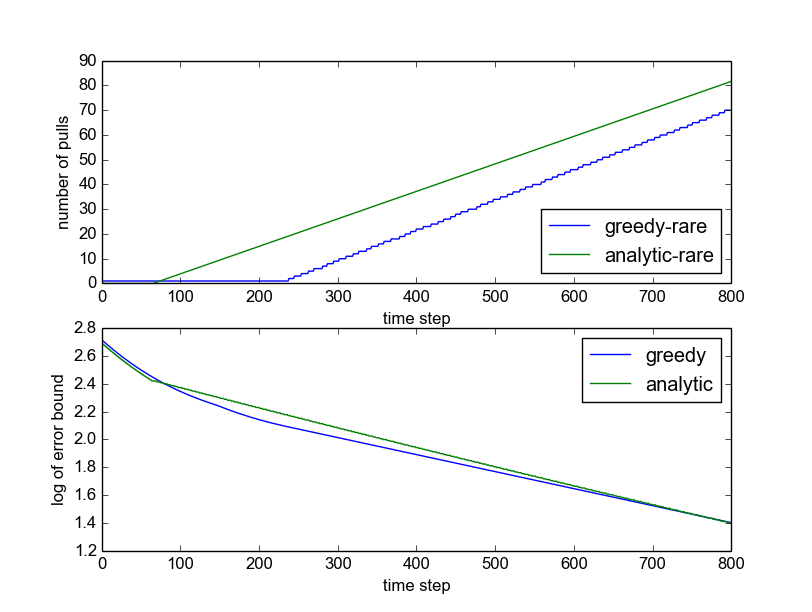
\includegraphics[width=.5\textwidth]{greedy_minimization_close}
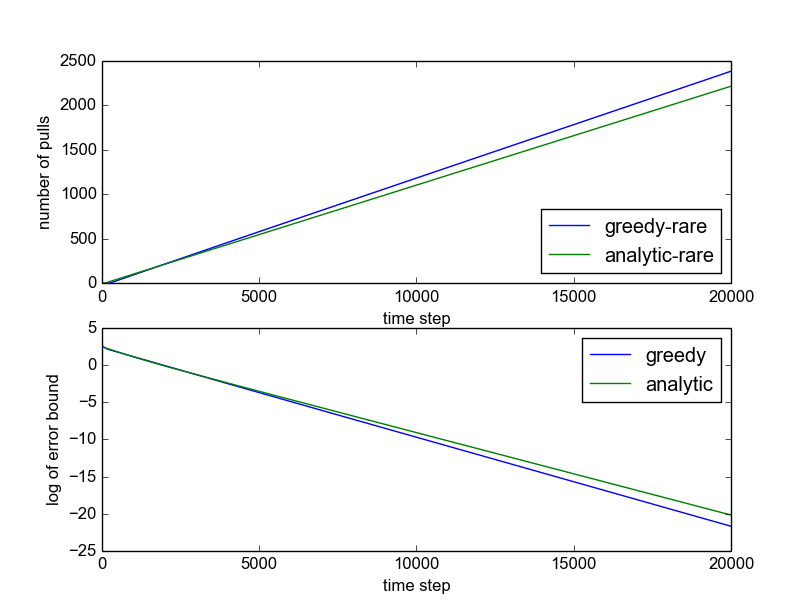
\includegraphics[width=.5\textwidth]{greedy_minimization}


Ok - so when we have many unbalanced variables, we assign almost all actions to the arms corresponding to the rare side. However, this will still be $< h/N$ which is only a factor of $2$ better than uniform assignment. Doing something smarter than uniform assignment will make more difference where we have a only a few unbalanced variables. In this case - smart assignment will lead to bounds almost as tight as the perfectly balanced case. Uniform assignment may yield solutions that are almost as bad as the worst case. (still better than without using the structure at all)

I still need to cover more fractional $q$'s... 



What about if I repeated one of the above analysis but let the unbalanced q = .75?

What can I say overall about worst/best cases/any symmetries in the problem??? Do these solutions lead to the terms in the exponentials being similar?

Goal is to choose something that will give us a simple bound and will be ok for the worst case. Its still not entirely clear to me what the worst case will be - after all it depends on the way you assign to $\tau$.

What happens if we assume $\sum_{a\neq i} c_a$ is constant ... this is reasonable if $N$ is large 

When you look at each term in $c_a$, its maximized if we play the arms according to their natural probabilities. If the arm is balanced, this will also minimize the sum of the two terms for doing $x_i = 0$ and $x_i = 1$. If the arm is unbalanced, then we have to trade of balancing this sum versus contributing to the sum of $c_a$. Consider just how bad the sum of $c_a$ can be even if we focus entirely on balancing the two terms ... maybe its already enough.

Fundamentally the relationship between arms is complex. Its not that we get any direct link from one arm to another - rather pairs of actions tell us something about other arms.   


Ok, suppose we spend half our actions, $\frac{h}{2}$, observing - that is selecting variables on which to act uniformly and setting them according to their natural probabilities. This contributes $\frac{h}{2N}$ to each $c_a$. So $\sum_{i\neq a} c_a \sim \frac{h}{2}$ provided $N-1 \sim N$. We don't allocate any more pulls to the more likely arm associated with each variable (this is at most a factor of 2 two few pulls). We now decide how to spend the remaining budget.

We can assume without loss of generality that $q_i \in [0,\frac{1}{2}]$ and $q_1 \leq ... \leq q_N$

\eqn{
f(\boldsymbol{\tau})  \leq  \sum_{i=1}^N e^{-A ( \tau_{i1} + q_{i}^2 \frac{h}{2})}+\sum_{i=1}^N e^{-A (\frac{h}{8})}
}

Evenly balanced allocation is $\frac{h}{2N}$. For those arms for which $q_i^2 \geq \frac{1}{N}$ they will already get this much information during the observe phase so we will not allocate them any more (again - at worst a factor or 2 two few). Lets just allocate the remainder evenly. So let $m = min\{m:m\leq N,\frac{1}{m} \leq q_m \}$

\eqn{
f(\boldsymbol{\tau})  \leq  \sum_{i=1}^N e^{-A ( \tau_{i1} + q_{i}^2 \frac{h}{2})}+N e^{-A (\frac{h}{8})}
}


\pagebreak

\subsection{Option 2: Some measure of information gain}

\subsection{Option 3: Three stage algorithm}
\begin{enumerate}
\item Observe randomly
\item Play low probability arms
\item Pick best and exploit
\end{enumerate}





